\subsection{Braided monoidal structure}

In the following we will construct a braided monoidal structure obtained from a op-fibration over $\Ex$.
To do so, we will need to choose paths in $\Ex$ on various occasions. We will refrain from specifying
the paths in detail but rather describe the paths enough to understand from which homotopy class we
choose a path and why some are homotopy equivalent. Also, we do not care much about the size of the
disks as we can expand and shrink them continuously as needed.
So, for this section we assume a basic topological understanding which for instance can be found in \cite{munkres}

\begin{rem}
    Let us recall the definition of $\Ex$. For each $n \in \N$ we have an object $\langle n \rangle$. 
    A mophism $\langle n \rangle \to \langle m \rangle$ in $\Ex$ consists of a morphism 
    $\alpha \colon \langle n \rangle \to \langle m \rangle$ in $\Fin$ and a collection of configurations
    $$\{c_j \in \E_2(|\alpha^{-1}(j)|)\}_{1 \leq j \leq m}$$
    where each configuration is labeled by $\alpha^{-1}(j))$.
    So for example, 
    \begin{align*}
        \alpha \colon \langle 3 \rangle &\to \langle 2 \rangle \\
        1 &\mapsto 1 \\
        2 &\mapsto 2 \\
        3 &\mapsto 1 \\
    \end{align*}
    together with the configurations
    \begin{center}
    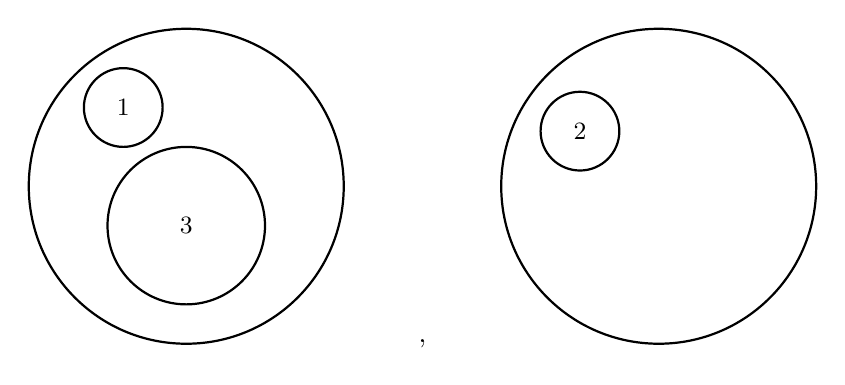
\begin{tikzpicture}
                        % First element (left)
                        \draw[thick] (-3,0) circle (2);
                        \draw[thick] (-3.8, 1) circle (0.5);
                        \draw[thick] (-3, -0.5) circle (1);
                        \node at (-3.8, 1) {\small $1$};
                        \node at (-3, -0.5) {\small $3$};
                        \node at (0,-2) {,};
                        % Second element (right)
                        \draw[thick] (3,0) circle (2);
                        \draw[thick] (2,0.7) circle (0.5);
                        \node at (2,0.7) {\small $2$};
        \end{tikzpicture}
    \end{center}
    We denote the trivial configuration with label $x$ by $\id^x \in \E_2(1)$.
\end{rem}

We will follow now the same approach as in the symmetic monoidal case in section \ref{sec:operads}, i.e. we will define a category $\Cotimes$ and a functor $\pi \colon \Cotimes \to \Ex$ such that $\pi$ is a op-fibration and the fibers of $\pi$ are given by the categories $\C^n \coloneqq \Cotimes_{\langle n \rangle}$ for $n \geq 1$.


\begin{defin}
    An $\E_2$-operad is a category $\Cotimes$ with a functor
    \[
        \Cotimes \to \Ex
    \]
    satisfying
        \begin{enumerate}[(M1)]
            \item \textbf{Op-fibration condition:} The functor $\pi$ is a op-fibration.
            \item \textbf{Segal condition:} For $\C \coloneqq \Cotimes_{\langle 1 \rangle}$, we have $\Cotimes_{\langle n \rangle} \cong \C^n$ for all $n \geq 1$. 
        \end{enumerate}

\end{defin}



So for the next part, let $\pi \colon \Cotimes \to \Ex$ be a $\E_2$-operad and we denote $\C \coloneqq \Cotimes_{\langle 1 \rangle}$.
In the following section we aim to define a braided monoidal structure on $\C$.
First, note that for a diagram in $\Ex$ of the following form
\[
    \begin{tikzcd}
        \langle n \rangle \arrow[r, "c_1"] \arrow[rd, "c_2"] & \langle 1 \rangle \arrow[d, "\id"] \\
                                                            & \langle 1 \rangle                                                               
    \end{tikzcd}
\]
with $c_1$ and $c_2$ being configurations in $\E_2(n)$, commutativity means choosing a path from $c_1$ to $c_2$.
Let $\beta$ denote the following morphism in $\Ex$
     \begin{align*}
         \beta \colon \langle 2 \rangle &\to \langle 2 \rangle \\
         1 &\mapsto 2 \\
         2 &\mapsto 1. \\
     \end{align*}
with the trivial collection $(\id^2, \id^1)$.
Further, let 
\begin{align*}
    \mu \colon \langle 2 \rangle &\to \langle 1 \rangle \\
    1 &\mapsto 1 \\
    2 &\mapsto 1 \\
\end{align*}
be the morphism with the following configuration which we refer to as the 
basepoint configuration in $\E_2(2)$:


\begin{center}
    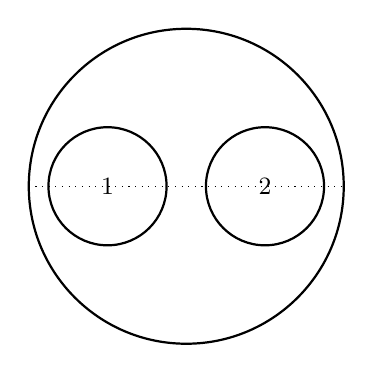
\begin{tikzpicture}
                        % First element (left)
                        \node at (1, 0) {\small $2$};
                        \node at (-1, 0) {\small $1$};
                        
                        \draw[thick] (0,0) circle (2);
                        \draw[thick] (1, 0) circle (0.75);
                        \draw[thick] (-1, 0) circle (0.75);
                        \draw[dotted](-2, 0)--(2, 0);       
        \end{tikzpicture}
\end{center}

Since $\pi$ satisfies the op-fibration condition (M1) and the Segal condition (M2), we have that for any $(A,B) \in \C^2 \cong \Cotimes_{\langle 2 \rangle}$ 
there is a cocartesian lift $(A,B) \to A \otimes B$. The cocartesian property ensures that the choice is 
unique up to isomorphism.
So, we obtain a well-defined functor
\[
    \otimes \colon \C^2 \to \C.
\]

Further, we consider the following diagramm in $\Ex$
\[    
    \begin{tikzcd}
        \langle 2 \rangle \arrow[r, "\beta"] \arrow[d, "\mu"] & \langle 2 \rangle \arrow[d, "\mu"] \\
        \langle 1 \rangle  \arrow[r, dashed]                  & \langle 1 \rangle.                 
    \end{tikzcd}
\]
Filling the diagram, i.e. giving commutativity means choosing a path 
from the basepoint configuration corresponding to $\mu$ 
to the twisted basepoint configuration corresponding to $\mu \circ \beta$. 
We choose this to be the half twist.

\begin{center}
    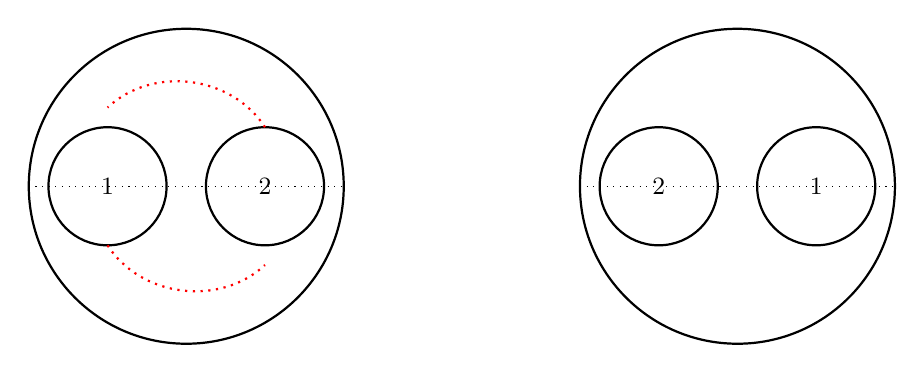
\begin{tikzpicture}
                        % basepoint
                        \node at (1, 0) {\small $2$};
                        \node at (-1, 0) {\small $1$};
                        
                        \draw[thick] (0,0) circle (2);
                        \draw[thick] (1, 0) circle (0.75);
                        \draw[thick] (-1, 0) circle (0.75);
                        \draw[dotted](-2, 0)--(2, 0);
                        \draw[thick, dotted, red] (-1, -0.75) to [bend right=50] (1, -1);
                        \draw[thick, dotted, red] (1, 0.75) to [bend right=50] (-1, 1);

                        \node at (3.5, 0) {$\rightsquigarrow$};
                        
                        % twisted basepoint
                        \node at (8, 0) {\small $1$};
                        \node at (6, 0) {\small $2$};
                        
                        \draw[thick] (7,0) circle (2);
                        \draw[thick] (8, 0) circle (0.75);
                        \draw[thick] (6, 0) circle (0.75);
                        \draw[dotted](5, 0)--(9, 0);  
                        
        \end{tikzpicture}
\end{center}

Since $\pi$ is an op-fibration, we obtain for a pair $(A,B)$ a cocartesian morphism 
$\beta' \colon (A,B) \to (B,A)$ in $\C^2$ with $\pi(\beta')=\beta$.


Since $\otimes$ and $\beta'$ are cocartesian and composites of cocartesian morphism are again 
cocartesian, we can lift the diagram in both directions:
\[    
    \begin{tikzcd}
        \langle 2 \rangle \arrow[r, "\beta"] \arrow[d, "\mu"] & \langle 2 \rangle \arrow[d, "\mu"] \\
        \langle 1 \rangle  \arrow[r, dashed]                  & \langle 1 \rangle.                 
    \end{tikzcd}
\]
and obtain two commuting diagram in $\Cotimes$:
\[
\begin{tikzcd}
{(A,B)} \arrow[r, "\beta"] \arrow[d, "\otimes"] & {(B,A)} \arrow[d, "\otimes"]                        \\
A \otimes B \arrow[r, "b", dashed, shift left]  & B \otimes A \arrow[l, "b^{-1}", dashed, shift left]
\end{tikzcd}
\]
The morphism $b$ is the induced morphism from the cocartesian morphism $\otimes$ while $b^{-1}$ 
is induces by $\otimes \circ \beta'$. 
They are inverse to one another since lifts are unique.

The induced morphism $b$ is a unique isomorphism due to the fact that $\otimes$ and $\beta$ are cocartesian morphisms.
Note, that for a different choice of path instead of the half twist, we would obtain a
different braiding. So, this choice is essential for our construction.

For the associator we consider the following diagram in $\Ex$:
    \[
    \begin{tikzcd}
        \langle 3 \rangle \arrow[r, "\tau_2^3"] \arrow[d, "\tau^3_1"] & \langle 2 \rangle \arrow[d] \\
        \langle 2 \rangle \arrow[r]                                   & \langle 1 \rangle          
    \end{tikzcd}
    \]
    where the associated configurations are either the trivial configuration or the basepoint configuration.
    To fill the diagram, we choose a path $\gamma$ that only translates the middle points of the disks along the horizontal line and shrinks or expands the disks as needed.


 



    \begin{center}
        \begin{tikzpicture}
                        % First element (left)
                        \node at (-1, 0) {\small $1$};
                        \node at (0.625, 0) {\small $2$};
                        \node at (1.375, 0) {\small $3$};
                        \draw[thick] (0,0) circle (2);
                        \draw[thick] (-1, 0) circle (0.75);
                        \draw[thick] (0.625, 0) circle (0.275);
                        \draw[thick] (1.375, 0) circle (0.275);
                        \draw[dotted] (1, 0) circle (0.75);
                        \draw[dotted](-2, 0)--(2, 0);

                        \node at (3.5, 0) {$\overset{\gamma}{\rightsquigarrow}$};

                        % Second element (left)
                        \node at (5.625, 0) {\small $1$};
                        \node at (6.375, 0) {\small $2$};
                        \node at (8, 0) {\small $3$};
                        \draw[thick] (7,0) circle (2);
                        \draw[dotted] (6, 0) circle (0.75);
                        \draw[thick] (6.325, 0) circle (0.275);
                        \draw[thick] (5.675, 0) circle (0.275);
                        \draw[thick] (8, 0) circle (0.75);
                        \draw[dotted](5, 0)--(9, 0);     
        \end{tikzpicture}
    \end{center}

Again using the op-fibration condition (M1) property of $\pi$ we obtain a commuting diagram in $\Cotimes$
\[
\begin{tikzcd}
{(A \otimes B, C)} \arrow[d, "\otimes"] & {(A,B,C)} \arrow[r, "{(\id, \otimes)}"] \arrow[l, "{(\otimes, \id)}"'] & {(A, B \otimes C)} \arrow[d, "\otimes"] \\
(A \otimes B) \otimes C \arrow[rr, "a"] &                                                                        & A \otimes (B \otimes C)                
\end{tikzcd}
\]

Similarily to proposition \ref{SymMonBijection}, the tensor unit is given by the unique morphism 
$\eta \colon \langle 0 \rangle \to \langle 1 \rangle$ in $\Ex$ 
which induces a functor $\Cotimes_{\langle 0 \rangle} \to \C$ giving us a tensor unit $\mathbf{1}$.

\begin{prop}
    The category $\C$ equipped with $(\otimes, b, a, \mathbf{1})$ defines a braided monoidal category.
\end{prop}

\begin{proof}
    First, we observe that the associator refers to $\E_1$ being embedded into $\E_2$ along the horizontal line.
    \todo{picture of $E_1$ in $E_2$?}
    So, the pentagon identity holds as $\E_1$ is the associative operad.
    \todo{include a proof here if spare time}
    The unitality condition holds analoguously to the proof of proposition \ref{SymMonBijection} using the Segal condition.
    Hence, we focus on verifying the hexagon identities
    \begin{enumerate}
        \item 
        \[
            \begin{tikzcd}
                                                                                & A \otimes (B \otimes C) \arrow[r, "b"] & (B \otimes C) \otimes A  \arrow[rd, "a"]            &                         \\
            (A \otimes B) \otimes C \arrow[ru, "a"] \arrow[rd, "b \otimes \id"] &                                        &                                                     & B \otimes (C \otimes A) \\
                                                                                & (B \otimes A) \otimes C \arrow[r, "a"] & B \otimes (A \otimes C) \arrow[ru, "\id \otimes b"] &                        
            \end{tikzcd}
        \]
        \item 
        \[
            \begin{tikzcd}
                                                                                & (A \otimes B) \otimes C \arrow[r, "b"] & C \otimes (A \otimes B) \arrow[rd, "a"]             &                         \\
            A \otimes (B \otimes C) \arrow[ru, "a"] \arrow[rd, "\id \otimes b"] &                                        &                                                     & (C \otimes A) \otimes B \\
                                                                                & A \otimes (C \otimes B) \arrow[r, "a"] & (A \otimes C) \otimes B \arrow[ru, "b \otimes \id"] &                        
            \end{tikzcd}
        \]
    \end{enumerate}
    Each edge in the hexagon diagrams refers to a commuting diagram in $\Ex$ of the form

    \[
        \begin{tikzcd}
                                            & \langle 3 \rangle \arrow[ldd, "c_{A \otimes B \otimes C}"', bend right] \arrow[d, "c_{(A \otimes B) \otimes C}" description] \arrow[rdd, "c_{C \otimes (A\otimes B)}", bend left] &                   \\
                                            & \langle 1 \rangle \arrow[ld, "\id"] \arrow[rd, "\id"']                                                                                                                            &                   \\
        \langle 1 \rangle \arrow[rr, "\id"] &                                                                                                                                                                                   & \langle 1 \rangle
        \end{tikzcd}
    \]
   
    with configurations:
    \begin{center}
        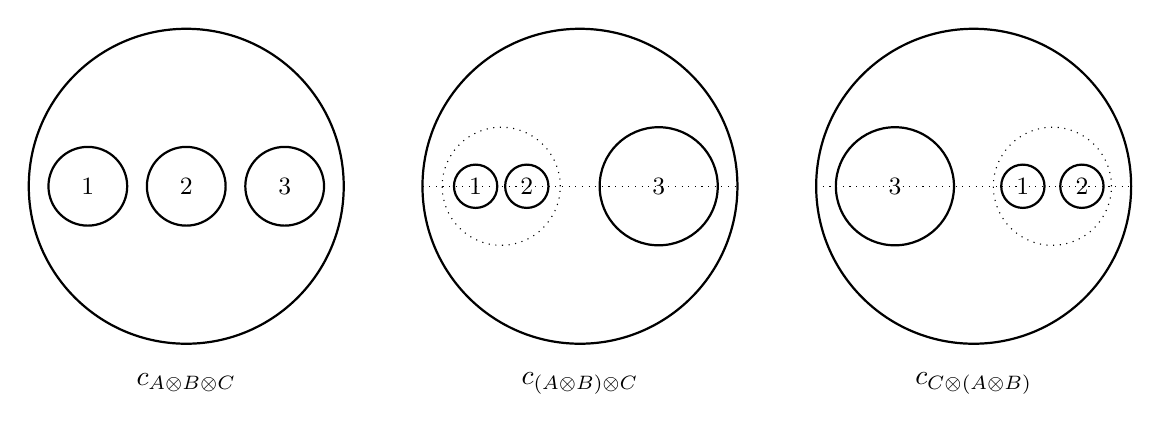
\begin{tikzpicture}
            \node at (0,-2.5) {$c_{(A \otimes B) \otimes C}$};
            \node at (-5,-2.5) {$c_{A \otimes B \otimes C}$};
            \node at (5,-2.5) {$c_{C \otimes (A \otimes B)}$};


            % left configuration (left)
            \draw[thick] (-5,0) circle (2);
            \draw[thick] (-3.75, 0) circle (0.5);
            \draw[thick] (-5, 0) circle (0.5);
            \draw[thick] (-6.25, 0) circle (0.5);
            \node at (-6.25, 0) {\small $1$};
            \node at (-5, 0) {\small $2$};
            \node at (-3.75, 0) {\small $3$};

            % second configuration (middle)
            \node at (-0.675, 0) {\small $2$};
            \node at (-1.325, 0) {\small $1$};
            \node at (1, 0) {\small $3$};
            \draw[thick] (0,0) circle (2);
            \draw[dotted] (-1, 0) circle (0.75);
            \draw[thick] (-0.675, 0) circle (0.275);
            \draw[thick] (-1.325, 0) circle (0.275);
            \draw[thick] (1, 0) circle (0.75);
            \draw[dotted](-2, 0)--(2, 0);

            % third element (right)
            \node at (4, 0) {\small $3$};
            \node at (5.625, 0) {\small $1$};
            \node at (6.375, 0) {\small $2$};
            \draw[thick] (5,0) circle (2);
            \draw[thick] (4, 0) circle (0.75);
            \draw[thick] (5.625, 0) circle (0.275);
            \draw[thick] (6.375, 0) circle (0.275);
            \draw[dotted] (6, 0) circle (0.75);
            \draw[dotted](3, 0)--(7, 0);  

        \end{tikzpicture}
    \end{center}
    \todo{describe one commuting tetrahedron in detail. Rest analogpously leading tot he following diagram...}
    The commutativity of the triangle diagrams on the side mean choosing a path from one configuration to 
    another while filling the tetrahedron in $\Ex$ means having a homotopy between the the different paths. 
    As it turns out we do not make any new choices of paths. The paths are induced by the half twist we chose to define $\otimes$.
    \todo{give details. that $\langle 3 \rangle \to \langle 1 \rangle$ factros through $\langle 2  \rangle$ etc}
    The paths are chosen such that the configurations are homotopic to the basepoint configuration \todo{define basepoint config earlier}. 

    \begin{center}
        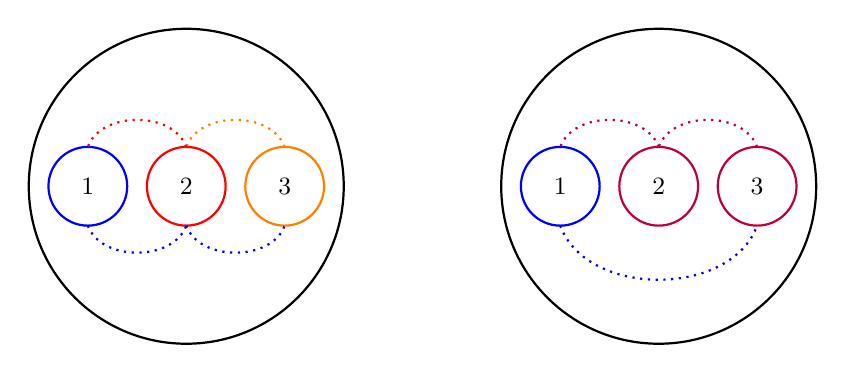
\begin{tikzpicture}
            %arrow
            \node at (-2, -0) {$\rightsquigarrow$};

            % left side paths
            \draw[thick] (-5,0) circle (2);
            \draw[thick, orange] (-3.75, 0) circle (0.5);
            \draw[thick, red] (-5, 0) circle (0.5);
            \draw[thick, blue] (-6.25, 0) circle (0.5);
            \node at (-6.25, 0) {\small $1$};
            \node at (-5, 0) {\small $2$};
            \node at (-3.75, 0) {\small $3$};

            %right side paths
            \draw[thick] (1,0) circle (2);
            \draw[thick, purple] (2.25, 0) circle (0.5);
            \draw[thick, purple] (1, 0) circle (0.5);
            \draw[thick, blue] (-0.25, 0) circle (0.5);
            \node at (-0.25, 0) {\small $1$};
            \node at (1, 0) {\small $2$};
            \node at (2.25, 0) {\small $3$};

            % paths
            \draw[dotted, thick, orange] (-3.75, 0.5) to [bend right=70] (-5, 0.5);
            \draw[dotted, thick, red] (-5, 0.5) to [bend right=70] (-6.25, 0.5);
            \draw[dotted, thick, blue] (-6.25, -0.5) to [bend right=70] (-5, -0.5);
            \draw[dotted, thick, blue] (-5, -0.5) to [bend right=70] (-3.75, -0.5);
            \draw[dotted, thick, purple] (2.25, 0.5) to [bend right=70] (1, 0.5);
            \draw[dotted, thick, purple] (1, 0.5) to [bend right=70] (-0.25, 0.5);
            \draw[dotted, thick, blue] (-0.25, -0.5) to [bend right=70] (2.25, -0.5);
        \end{tikzpicture}
    \end{center}

    \newpage
    
    The paths above are desribed by the following diagram which is the translation of the first hexagon identity to the corresponding configuration.
        \begin{center}
        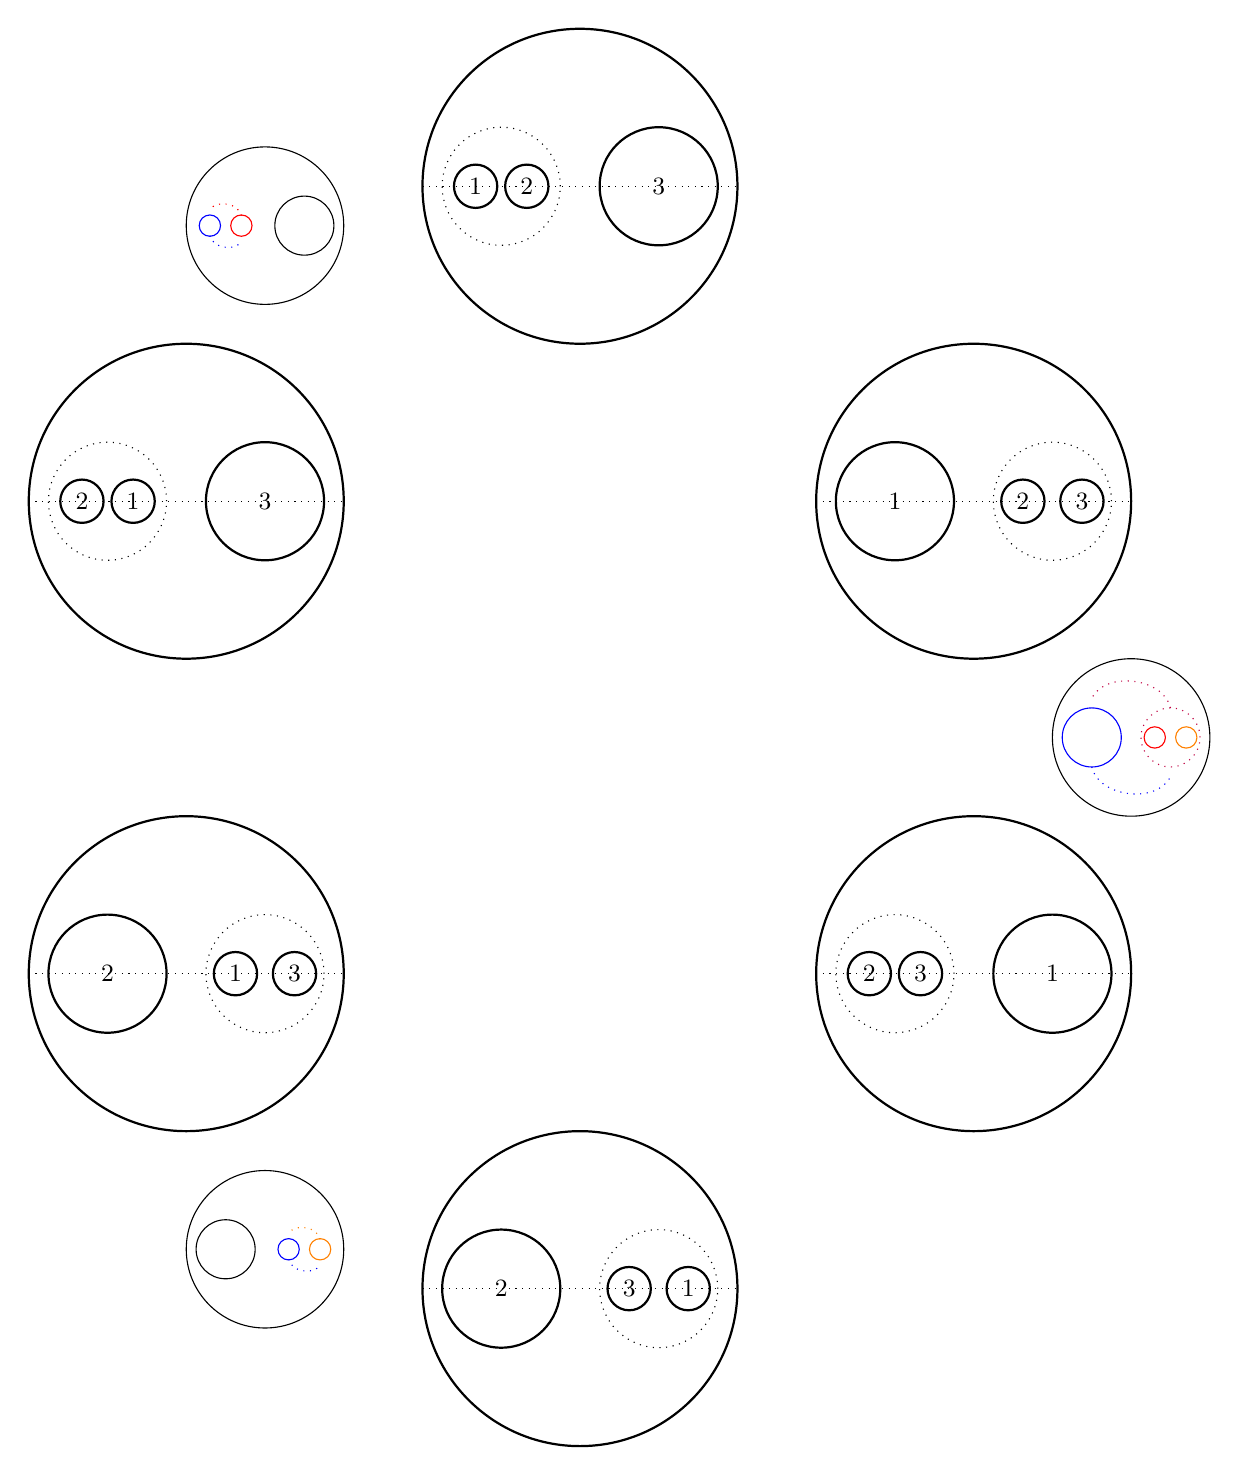
\begin{tikzpicture}
            %arrows
            \node at (-2.5, -2) {\rotatebox{-135}{$\rightsquigarrow$}};
            \node at (2.5, -2) {\rotatebox{-45}{$\rightsquigarrow$}};
            \node at (-5, -7) {\rotatebox{-90}{$\rightsquigarrow$}};
            \node at (5, -7) {\rotatebox{-90}{$\rightsquigarrow$}};
            \node at (2.5, -12) {\rotatebox{-135}{$\rightsquigarrow$}};
            \node at (-2.5, -12) {\rotatebox{-45}{$\rightsquigarrow$}};

            % top
            \node at (-0.675, 0) {\small $2$};
            \node at (-1.325, 0) {\small $1$};
            \node at (1, 0) {\small $3$};
            \draw[thick] (0,0) circle (2);
            \draw[dotted] (-1, 0) circle (0.75);
            \draw[thick] (-0.675, 0) circle (0.275);
            \draw[thick] (-1.325, 0) circle (0.275);
            \draw[thick] (1, 0) circle (0.75);
            \draw[dotted](-2, 0)--(2, 0);

            % right first
            \node at (4, -4) {\small $1$};
            \node at (5.625, -4) {\small $2$};
            \node at (6.375, -4) {\small $3$};
            \draw[thick] (5,-4) circle (2);
            \draw[thick] (4, -4) circle (0.75);
            \draw[thick] (5.625, -4) circle (0.275);
            \draw[thick] (6.375, -4) circle (0.275);
            \draw[dotted] (6, -4) circle (0.75);
            \draw[dotted](3, -4)--(7, -4); 
                 
            % left first
            \node at (-5.675, -4) {\small $1$};
            \node at (-6.325, -4) {\small $2$};
            \node at (-4, -4) {\small $3$};
            \draw[thick] (-5,-4) circle (2);
            \draw[dotted] (-6, -4) circle (0.75);
            \draw[thick] (-5.675, -4) circle (0.275);
            \draw[thick] (-6.325, -4) circle (0.275);
            \draw[thick] (-4, -4) circle (0.75);
            \draw[dotted](-7, -4)--(-3, -4);

            % right second
            \node at (4.325, -10) {\small $3$};
            \node at (3.675, -10) {\small $2$};
            \node at (6, -10) {\small $1$};
            \draw[thick] (5,-10) circle (2);
            \draw[dotted] (4, -10) circle (0.75);
            \draw[thick] (4.325, -10) circle (0.275);
            \draw[thick] (3.675, -10) circle (0.275);
            \draw[thick] (6, -10) circle (0.75);
            \draw[dotted](3, -10)--(7, -10);

            % left second
            \node at (-6, -10) {\small $2$};
            \node at (-4.375, -10) {\small $1$};
            \node at (-3.625, -10) {\small $3$};
            \draw[thick] (-5,-10) circle (2);
            \draw[thick] (-6, -10) circle (0.75);
            \draw[thick] (-4.375, -10) circle (0.275);
            \draw[thick] (-3.625, -10) circle (0.275);
            \draw[dotted] (-4, -10) circle (0.75);
            \draw[dotted](-7, -10)--(-3, -10);

            %bottom
            \node at (-1, -14) {\small $2$};
            \node at (0.625, -14) {\small $3$};
            \node at (1.375, -14) {\small $1$};
            \draw[thick] (0,-14) circle (2);
            \draw[thick] (-1, -14) circle (0.75);
            \draw[thick] (0.625, -14) circle (0.275);
            \draw[thick] (1.375, -14) circle (0.275);
            \draw[dotted] (1, -14) circle (0.75);
            \draw[dotted](-2, -14)--(2, -14);

            % paths visualisation #1
            \draw (-4,-0.5) circle (1);
            %\draw[dotted] (-1, 0) circle (0.375);
            \draw[blue] (-4.7, -0.5) circle (0.13525);
            \draw[red] (-4.3, -0.5) circle (0.13525);
            \draw (-3.5, -0.5) circle (0.375);
            \draw[dotted, red] (-4.3, -0.375) to [bend right=70] (-4.7, -0.3);
            \draw[dotted, blue] (-4.7, -0.625) to [bend right=70] (-4.3, -0.7);

            % paths visualisation #2
            \draw (-4,-13.5) circle (1);
            %\draw[dotted] (-1, 0) circle (0.375);
            \draw[orange] (-3.3, -13.5) circle (0.13525);
            \draw[blue] (-3.7, -13.5) circle (0.13525);
            \draw (-4.5, -13.5) circle (0.375);
            \draw[dotted, blue] (-3.7, -13.625) to [bend right=70] (-3.3, -13.7);
            \draw[dotted, orange] (-3.3, -13.375) to [bend right=70] (-3.7, -13.3);

            % paths visualisation #3
            \draw (7,-7) circle (1);
            \draw[dotted, purple] (7.5, -7) circle (0.375);
            \draw[orange] (7.7, -7) circle (0.13525);
            \draw[red] (7.3, -7) circle (0.13525);
            \draw[blue] (6.5, -7) circle (0.375);
            \draw[dotted, purple] (7.5, -6.625) to [bend right=70] (6.5, -6.5);
            \draw[dotted, blue] (6.5, -7.375) to [bend right=70] (7.5, -7.5);
        \end{tikzpicture}
    \end{center}

    \newpage

    For the second hexagon identity we consider the following diagram in $\Ex$:
    \begin{center}
        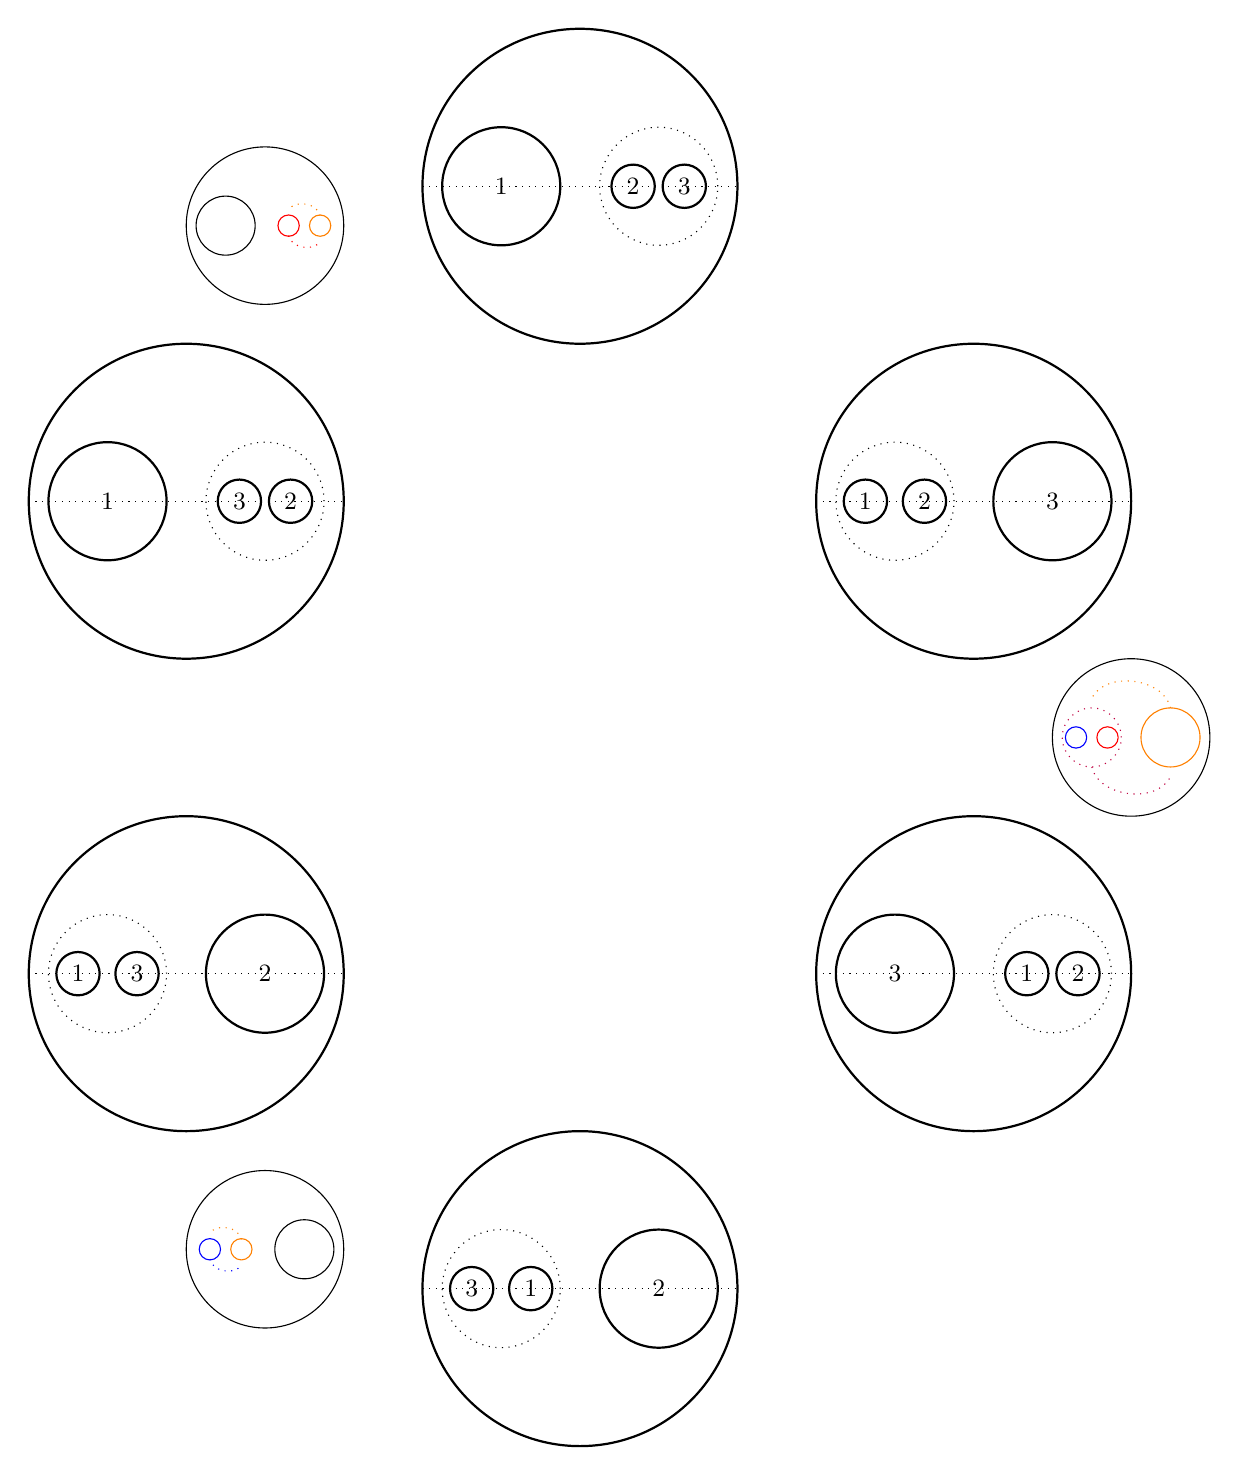
\begin{tikzpicture}
            %arrows
            \node at (-2.5, -2) {\rotatebox{-135}{$\rightsquigarrow$}};
            \node at (2.5, -2) {\rotatebox{-45}{$\rightsquigarrow$}};
            \node at (-5, -7) {\rotatebox{-90}{$\rightsquigarrow$}};
            \node at (5, -7) {\rotatebox{-90}{$\rightsquigarrow$}};
            \node at (2.5, -12) {\rotatebox{-135}{$\rightsquigarrow$}};
            \node at (-2.5, -12) {\rotatebox{-45}{$\rightsquigarrow$}};

            % top
            \node at (0.675, 0) {\small $2$};
            \node at (1.325, 0) {\small $3$};
            \node at (-1, 0) {\small $1$};
            \draw[thick] (0,0) circle (2);
            \draw[dotted] (1, 0) circle (0.75);
            \draw[thick] (0.675, 0) circle (0.275);
            \draw[thick] (1.325, 0) circle (0.275);
            \draw[thick] (-1, 0) circle (0.75);
            \draw[dotted](-2, 0)--(2, 0);

            % right first
            \node at (6, -4) {\small $3$};
            \node at (3.625, -4) {\small $1$};
            \node at (4.375, -4) {\small $2$};
            \draw[thick] (5,-4) circle (2);
            \draw[thick] (6, -4) circle (0.75);
            \draw[thick] (3.625, -4) circle (0.275);
            \draw[thick] (4.375, -4) circle (0.275);
            \draw[dotted] (4, -4) circle (0.75);
            \draw[dotted](3, -4)--(7, -4); 
                 
            % left first
            \node at (-3.675, -4) {\small $2$};
            \node at (-4.325, -4) {\small $3$};
            \node at (-6, -4) {\small $1$};
            \draw[thick] (-5,-4) circle (2);
            \draw[dotted] (-4, -4) circle (0.75);
            \draw[thick] (-3.675, -4) circle (0.275);
            \draw[thick] (-4.325, -4) circle (0.275);
            \draw[thick] (-6, -4) circle (0.75);
            \draw[dotted](-7, -4)--(-3, -4);

            % right second
            \node at (6.325, -10) {\small $2$};
            \node at (5.675, -10) {\small $1$};
            \node at (4, -10) {\small $3$};
            \draw[thick] (5,-10) circle (2);
            \draw[dotted] (6, -10) circle (0.75);
            \draw[thick] (6.325, -10) circle (0.275);
            \draw[thick] (5.675, -10) circle (0.275);
            \draw[thick] (4, -10) circle (0.75);
            \draw[dotted](3, -10)--(7, -10);

            % left second
            \node at (-4, -10) {\small $2$};
            \node at (-6.375, -10) {\small $1$};
            \node at (-5.625, -10) {\small $3$};
            \draw[thick] (-5,-10) circle (2);
            \draw[thick] (-4, -10) circle (0.75);
            \draw[thick] (-6.375, -10) circle (0.275);
            \draw[thick] (-5.625, -10) circle (0.275);
            \draw[dotted] (-6, -10) circle (0.75);
            \draw[dotted](-7, -10)--(-3, -10);

            %bottom
            \node at (1, -14) {\small $2$};
            \node at (-0.625, -14) {\small $1$};
            \node at (-1.375, -14) {\small $3$};
            \draw[thick] (0,-14) circle (2);
            \draw[thick] (1, -14) circle (0.75);
            \draw[thick] (-0.625, -14) circle (0.275);
            \draw[thick] (-1.375, -14) circle (0.275);
            \draw[dotted] (-1, -14) circle (0.75);
            \draw[dotted](-2, -14)--(2, -14);

            % paths visualisation #1
            \draw (-4,-0.5) circle (1);
            %\draw[dotted] (-1, 0) circle (0.375);
            \draw[red] (-3.7, -0.5) circle (0.13525);
            \draw[orange] (-3.3, -0.5) circle (0.13525);
            \draw (-4.5, -0.5) circle (0.375);
            \draw[dotted, orange] (-3.3, -0.375) to [bend right=70] (-3.7, -0.3);
            \draw[dotted, red] (-3.7, -0.625) to [bend right=70] (-3.3, -0.7);

            % paths visualisation #2
            \draw (-4,-13.5) circle (1);
            %\draw[dotted] (-1, 0) circle (0.375);
            \draw[orange] (-4.3, -13.5) circle (0.13525);
            \draw[blue] (-4.7, -13.5) circle (0.13525);
            \draw (-3.5, -13.5) circle (0.375);
            \draw[dotted, blue] (-4.7, -13.625) to [bend right=70] (-4.3, -13.7);
            \draw[dotted, orange] (-4.3, -13.375) to [bend right=70] (-4.7, -13.3);

            % paths visualisation #3
            \draw (7,-7) circle (1);
            \draw[dotted, purple] (6.5, -7) circle (0.375);
            \draw[red] (6.7, -7) circle (0.13525);
            \draw[blue] (6.3, -7) circle (0.13525);
            \draw[orange] (7.5, -7) circle (0.375);
            \draw[dotted, purple] (6.5, -7.375) to [bend right=70] (7.5, -7.5);
            \draw[dotted, orange] (7.5, -6.625) to [bend right=70] (6.5, -6.5);
        \end{tikzpicture}
    \end{center}

    \newpage

    The resulting paths are again homotopy equivalent and therefore the second hexagon identity holds.
    \begin{center}
        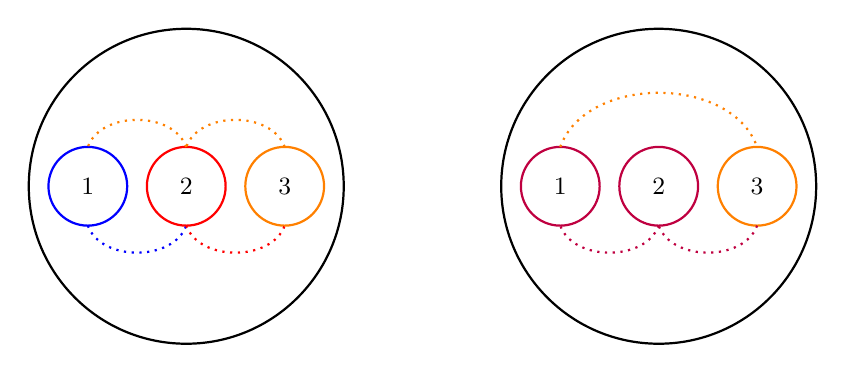
\begin{tikzpicture}
            %arrows
            \node at (-2, -0) {$\rightsquigarrow$};

            % left side paths
            \draw[thick] (-5,0) circle (2);
            \draw[thick, orange] (-3.75, 0) circle (0.5);
            \draw[thick, red] (-5, 0) circle (0.5);
            \draw[thick, blue] (-6.25, 0) circle (0.5);
            \node at (-6.25, 0) {\small $1$};
            \node at (-5, 0) {\small $2$};
            \node at (-3.75, 0) {\small $3$};

            %right side paths
            \draw[thick] (1,0) circle (2);
            \draw[thick, orange] (2.25, 0) circle (0.5);
            \draw[thick, purple] (1, 0) circle (0.5);
            \draw[thick, purple] (-0.25, 0) circle (0.5);
            \node at (-0.25, 0) {\small $1$};
            \node at (1, 0) {\small $2$};
            \node at (2.25, 0) {\small $3$};

            % paths
            \draw[dotted, thick, orange] (-3.75, 0.5) to [bend right=70] (-5, 0.5);
            \draw[dotted, thick, orange] (-5, 0.5) to [bend right=70] (-6.25, 0.5);
            \draw[dotted, thick, blue] (-6.25, -0.5) to [bend right=70] (-5, -0.5);
            \draw[dotted, thick, red] (-5, -0.5) to [bend right=70] (-3.75, -0.5);
            \draw[dotted, thick, purple] (2.25, -0.5) to [bend left=70] (1, -0.5);
            \draw[dotted, thick, purple] (1, -0.5) to [bend left=70] (-0.25, -0.5);
            \draw[dotted, thick, orange] (-0.25, 0.5) to [bend left=70] (2.25, 0.5);
        \end{tikzpicture}
    \end{center}
    This concludes the proof that $\Ex$ induces a braided monoidal structure on $\C$.

\end{proof}


\subsection{Universal Covering of $\E_2$}

In this section we want to establish an operadic structure on the universal covering of $\E_2$.
First, we need to define what it means to be a universal covering of a topological operad.

\begin{defin}
    Let $\P$  be a topological operad. 
    A covering operad $\widetilde{\P}$ is a topological operad 
    such that there is a morphism of operads $c \colon \widetilde{\P} \to \P$ 
    where $c_n \colon \widetilde{\P}(n) \to \P(n)$ is a covering of $\P(n)$ for all $n \geq 1$.
\end{defin}

\begin{defin}
    Let $\P$ be a topological operad. A universal covering operad $\widetilde{\P}$ is a covering 
    operad that is universal in every degree $n \geq 1$.
\end{defin}

While the operadic structure requires labels in the sense that they are necessary to define the composition maps in
$\E_2$, they do not matter from a topologcial perspective. Hence, in this section we want to establish a universal 
covering of $\E_2$ without labels.
So, instead of $\E_2$ we will consider the quotient:
\[
    \E_2 \to \E_2 \slash S
\]
We identify configurations that only differ in their labels, i.e. we consider the quotient of $\E_2$ by the action of the symmetric group $S$ on the labels.
So, in $\Ex \slash S$ we identify $f, g \colon \langle n \rangle \to \langle m \rangle$ 
if there exists a commuting diagram in $\Ex$
\begin{center}
    \begin{tikzcd}
        \langle n \rangle \arrow[r, "f"] \arrow[d, "\sigma"] & \langle m \rangle \arrow[d, "\tau"] \\
        \langle n \rangle \arrow[r, "g"]                     & \langle m \rangle                  
    \end{tikzcd}
\end{center}
where $\sigma \in S_n$ and $\tau \in S_m$.

Before, we can find a universal covering of $\E_2 \slash S$, we need to choose basepoints in each configuration space.
So, for all $n \geq 1$ we choose the basepoint $b_n \in \E_2(n)$ to be the following configuration:
\begin{center}
    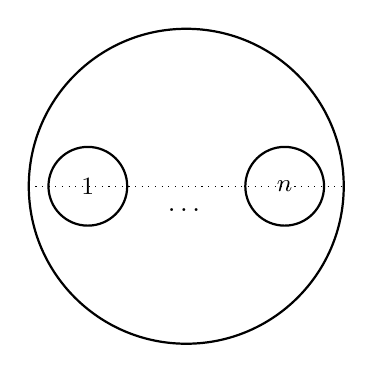
\begin{tikzpicture}
        %basepoint
        \draw[thick] (1,0) circle (2);
        \draw[thick] (2.25, 0) circle (0.5);
        \draw[thick] (-0.25, 0) circle (0.5);
        \node at (-0.25, 0) {\small $1$};
        \node at (1, -0.3) {\dots};
        \node at (2.25, 0) {\small $n$};
        \draw[dotted](-1, 0)--(3, 0);
    \end{tikzpicture}
\end{center}

Note that since $\E_2(n)$ is connected and simply connected then so is $\E_2 (n) \slash S_n$. 
Hence, it has a universal covering $\widetilde{\E_2}(n) \slash S_n$ which we define in the usual sense:
\[
    \widetilde{\E_2}(n) \slash S_n \coloneq \{ \gamma \colon [0,1] \to \E_2(n) \slash S_n \mid \gamma(0) = b_n \} 
    \slash \text{homotopy with fixed endpoints}
\]
with 
\begin{align*}
    p \colon \widetilde{\E_2}(n) \slash S_n &\to \E_2(n) \slash S_n \\
    \gamma &\mapsto \gamma(1)
\end{align*}
It is known that this in fact defines a universal covering of $\E_2(n) \slash S_n$.
Observe that for every $\gamma \in \widetilde{\E_2(n)} \slash S_n$ there is a commuting diagram in $\Ex$ for some $\sigma \in S_n$:
\begin{center}
    \begin{tikzcd}
        \langle n \rangle \arrow[d, "\sigma"'] \arrow[r, "c_n"] & \langle 1 \rangle \arrow[d, "\gamma", dashed] \\
        \langle n \rangle \arrow[r, "b_n"]                              & \langle 1 \rangle                            
    \end{tikzcd}
\end{center} 


However, we want to define an operadic structure on $\widetilde{\E_2} \slash S$ such that the 
covering is a morphism of operads.
\begin{prop}
    There is an operadic structure on $\widetilde{\E_2} \slash S$ such that the covering $p$ is a morphism 
    of operads.
\end{prop}

\begin{proof}
    Let 
    \[
        \gamma \colon \E_2(k) \times \E_2(j_1) \times \dots \times 
        \E_2(j_k) \to \E_2(j)
    \]
    be a composition map in $\E_2$.
    Then, we define a composition map in $\widetilde{\E_2}$
    \begin{align*}
        \gamma' \colon \widetilde{\E_2}(k) \times \widetilde{\E_2}(j_1) \times \dots \times 
        \widetilde{\E_2}(j_k) &\to \widetilde{\E_2}(j), \\
        % (\gamma_k, \gamma_{j_1}, \dots, \gamma_{j_k}) &\mapsto \gamma_k \circ (\gamma_{j_1}, \dots, 
        % \gamma_{j_k}) \circ \tau
    \end{align*}
    which we construct as follows:
    Let $(\bar{\alpha}, \alpha_1, \dots, \alpha_k) \in \widetilde{\E_2}(k) \times \widetilde{\E_2}(j_1) \times \dots \times 
        \widetilde{\E_2}(j_k)$
    with
        $$\alpha_l \colon b_{j_l} \to c_{j_l}$$
    and 
        $$\bar{\alpha} \colon b_k \to c_k.$$
    Then 
        \[
            \bar{\alpha} \circ (\alpha_1, \dots, \alpha_k)    
        \]
    denotes the path from $\gamma((b_k, b_{j_1}, \dots, b_{j_k}))$ to $\gamma(c_k, c_{j_1}, \dots, c_{j_k})$ 
    where we first apply 

    $$\alpha_l \colon b_{j_l} \to c_{j_l}$$

    on the configuration in the $l$-th disk of $b_k$ for all $1 \leq l \leq k$
    and then apply 

    $$\bar{\alpha} \colon b_k \to c_k$$

    on the configuration $b_k$.
    \begin{figure}[h!]
        
        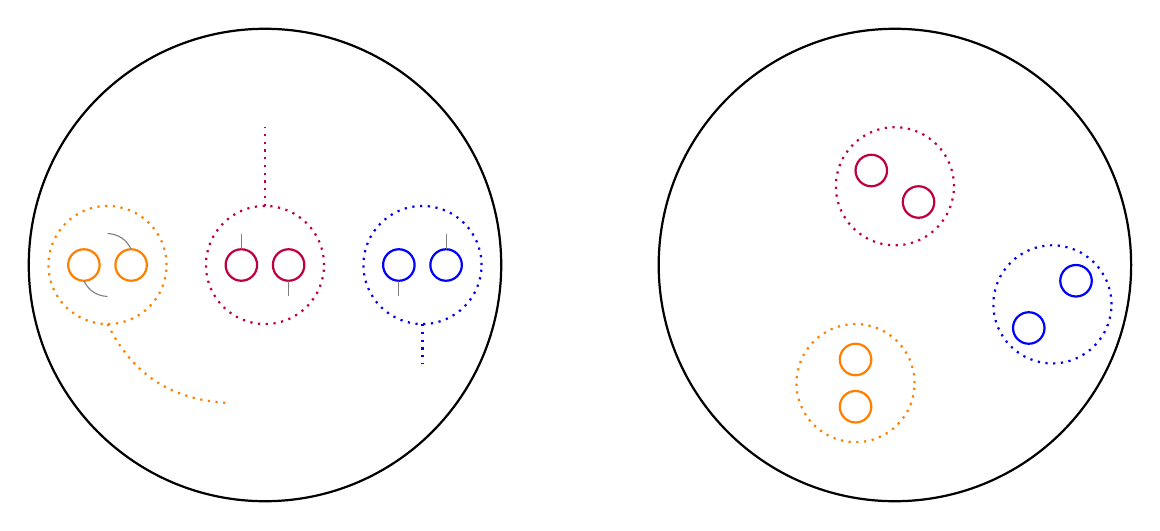
\begin{tikzpicture}
            \draw[thick] (-4,0) circle (3);
            \draw[dotted, thick, orange] (-6, 0) circle (0.75);
            \draw[thick, orange] (-6.3, 0) circle (0.2);
            \draw[thick, orange] (-5.7, 0) circle (0.2);
            \draw[dotted, thick, purple] (-4, 0) circle (0.75);
            \draw[thick, purple] (-4.3, 0) circle (0.2);
            \draw[thick, purple] (-3.7, 0) circle (0.2);
            \draw[dotted, thick, blue] (-2, 0) circle (0.75);
            \draw[thick, blue] (-2.3, 0) circle (0.2);
            \draw[thick, blue] (-1.7, 0) circle (0.2);

            \draw[thick] (4,0) circle (3);
            \draw[dotted,thick, orange] (3.5, -1.5) circle (0.75);
            \draw[thick, orange] (3.5, -1.2) circle (0.2);
            \draw[thick, orange] (3.5, -1.8) circle (0.2);
            \draw[dotted, thick, purple] (4, 1) circle (0.75);
            \draw[thick, purple] (3.7, 1.2) circle (0.2);
            \draw[thick, purple] (4.3, 0.8) circle (0.2);
            \draw[dotted,thick, blue] (6, -0.5) circle (0.75);
            \draw[thick, blue] (5.7, -0.8) circle (0.2);
            \draw[thick, blue] (6.3, -0.2) circle (0.2);

            %inner paths
            \draw[gray] (-6.3, -0.2) to [bend right=30] (-6, -0.4);   
            \draw[gray] (-5.7, 0.2) to [bend right=30] (-6, 0.4); 
            \draw[gray] (-4.3, 0.2) -- (-4.3, 0.4); 
            \draw[gray] (-3.7, -0.2) -- (-3.7, -0.4);  
            \draw[gray] (-2.3, -0.2) -- (-2.3, -0.4); 
            \draw[gray] (-1.7, 0.2) -- (-1.7, 0.4); 

            %outer paths to [bend right=70] (-3.75, -0.5);
            \draw[dotted, thick, orange] (-6, -0.75) to [bend right=30] (-4.5, -1.75);
            \draw[dotted, thick, purple] (-4., 0.75) -- (-4, 1.75);
            \draw[dotted, thick, blue] (-2, -0.75) -- (-2, -1.25);

            \node at (0,0) {$\rightsquigarrow$};
        \end{tikzpicture}
        \caption{example of $\bar{\alpha} \circ (\alpha_1, \dots, \alpha_3)$ 
        for $\bar{\alpha} \in \widetilde{E_2}(3)$ and $\alpha_1, \alpha_2, \alpha_3 \in \widetilde{E_2}(2)$}
    \end{figure}



    Further, let $\tau \in \E_1(j) \subset \E_2(j)$ be a path from $b_j$ to $\gamma((b_k, b_{j_1}, \dots, b_{j_k}))$
    that resizes and translates the disks along the horizontal axis. This path $\tau$ is unique up to homotopy.
    This generates the following commuting diagram in $\Ex$:
    \begin{center}
        \begin{tikzcd}
            \langle j \rangle  \arrow[rr, "{\gamma(c_k, c_{j_1}, \dots, c_{j_k})}"] \arrow[d, "S_j \ni"'] & & \langle 1 \rangle                                                                         \\
            \langle j \rangle  \arrow[d, "S_j \ni"'] \arrow[rr, "{\gamma(b_k, b_{j_1}, \dots, b_{j_k})}"] & & \langle 1 \rangle  \arrow[u, "{\bar{\alpha} \circ (\alpha_1, \dots, \alpha_k)}"', dashed] \\
            \langle j \rangle  \arrow[rr, "b_j"]                                                          & & \langle 1 \rangle  \arrow[u, "\tau"', dashed]                                            
        \end{tikzcd}
    \end{center}
    Therefore, we can set
    \[
        \gamma' ((\bar{\alpha}, \alpha_1, \dots, \alpha_k)) \coloneqq \bar{\alpha} \circ (\alpha_1, \dots, \alpha_k) \circ \tau
    \]
    Note, that for this definition is is necessary for the labels to be identified otherwise the path making the 
    lower square commute could possibly not be a translation along the horizontal axis.
    We observe, that this composition map is well-defined, since the path $\tau$ is unique up to homotopy and it is associative 
    due to the fact that the composition map in $\E_2$ is associative and composing paths is associaitve up to homotopy.
    Furthermore, we define a operadic unit
    \[
        \eta \colon \ast \to \widetilde{\E_2}(1)
    \]
    to be the trivial path of the trivial basepoint $b_1 \in \E_2(1)$. Clearly, this unit fulfills the unitality conditions.

    Finally, we need to show that the covering map $p \colon \widetilde{\E_2} \slash S \to \E_2 \slash S$ is a morphism of operads.
    For this, we need to show that the following diagram commutes for all $n \geq 1$:
    \begin{center}
        \begin{tikzcd}
            \widetilde{\E_2}(k) \slash S_k \times \widetilde{\E_2}(j_1) \slash S_{j_1} \times \dots \times \widetilde{\E_2}(j_k)\slash S_{j_k} \arrow[d, "\widetilde{\gamma}"] \arrow[rr, "p"] &  & \E_2(k)\slash S_k \times \E_2(j_1)\slash S_{j_1} \times \dots \times \E_2(j_k)\slash S_{j_k} \arrow[d, "\gamma"] \\
            \widetilde{\E_2}(j) \slash S_j \arrow[rr, "p"]                                                                                                                                     &  & \E_2(j) \slash S_j                                                                                              
        \end{tikzcd}
    \end{center}
    This is indeed the case, by definition of $\widetilde{\gamma}$ we have:
    \[
        p \circ \widetilde{\gamma} ((\bar{\alpha}, \alpha_1, \dots, \alpha_k)) = \gamma(c_k, c_{j_1}, \dots, c_{j_k})
    \]
    for $\gamma_l \colon b_{j_l} \to c_{j_l}$ and $\bar{\gamma} \colon b_k \to c_k$. Clearly, the unital condition is also met by definition:
    \begin{center}
        \begin{tikzcd}
                                        & \ast \arrow[ld, "\widetilde{\eta}"'] \arrow[rd, "\eta"] &                     \\
            \widetilde{\E_2}(1) \arrow[rr, "p"] &                                                         & \E_2(1)
        \end{tikzcd}
    \end{center}
    This concludes the proof that $\widetilde{\E_2} \slash S$  admits an operadic structure and the covering map is a morphism of operads.
\end{proof}

    This construction of an operadic structure on the universal covering of a topological operad can be given in a more general setting.
    Which we did not require at this point. But in lemma 4.1.12 in \cite{adrian} you can find a more general statement on how to construct an 
    operadic structure on the universal covering of a topological operad as long as there is an suboperad of $\E_1$ into the topological operad.

\subsubsection{Braid Action on $\widetilde{\E_2 \slash S}$}

As usual, there is a group action of of the fundamental group of $\E_2(n) \slash S(n)$ on its universal covering.
The fundamental group of $\E_2(n)$ is the $n$-th pure braid group $PB_n$. But since we forgot the labels when moving to
$\E_2(n) \slash S(n)$, we obtain now the full $n$-th braid group $B_n$.
We recall the generators of $B_n$ for all $1 \leq i < n$, $n \in \N$:
\begin{center}
    \begin{tikzpicture}
        \pic[
        braid/number of strands=6,
        braid/strand 2/.style={white},
        braid/strand 5/.style={white},
        name=coordinates,
        ] at (0,0) {braid={s_3}};
        \node[at=(coordinates-rev-2-e)] {$\dots$};
        \node[at=(coordinates-rev-3-e), below=3pt] {$i$};
        \node[at=(coordinates-rev-4-e), below=3pt] {$i+1$};
        \node[at=(coordinates-rev-5-e)] {$\dots$};
        \node[anchor=center] at (-0.5,-0.75) {$\sigma_i = \quad $};
    \end{tikzpicture}
\end{center}

We identify the generators with the homotopy class of the half twist of the $i$-th and $(i+1)$-th disk in
$\widetilde{\E_2 \slash S}$ which we will also denote by $\sigma_i$ from now on:
\begin{center}
    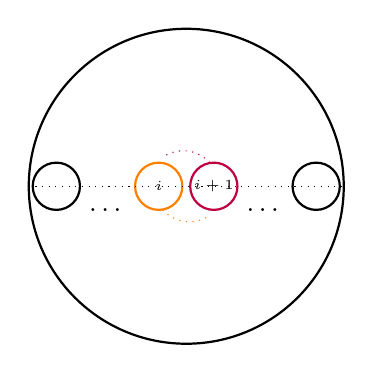
\begin{tikzpicture}
        %basepoint
        \draw[thick] (0,0) circle (2);
        \draw[thick] (1.65, 0) circle (0.3);
        \draw[thick, purple] (0.35, 0) circle (0.3);
        \draw[thick, orange] (-0.35, 0) circle (0.3);
        \draw[thick] (-1.65, 0) circle (0.3);
        % \node at (-0.25, 0) {\small $1$};
        \node at (1., -0.3) {\dots};
        \node at (-1., -0.3) {\dots};
        \node at (0.35, 0) {\tiny{$i+1$}};
        \node at (-0.35, 0) {\tiny{$i$}};

        \draw[dotted, purple](0.3, 0.3) [bend right=40] to (-0.3, 0.37);
        \draw[dotted, orange](-0.3, -0.3) [bend right=40] to (0.3, -0.37);
        \draw[dotted](-2, 0)--(2, 0);
    \end{tikzpicture}
\end{center}

Then, we obtain a braid action on $\widetilde{\E_2 \slash S}$.
Let $\alpha \colon b_n \to c$ be in $\widetilde{\E_2 \slash S}$ which is represented 
by the following diagram in $\Ex$ for some $\tau \in S_n$:

\begin{center}
    \begin{tikzcd}
        \langle n \rangle \arrow[r, "c"] \arrow[d, "\tau"']         & \langle 1 \rangle                                   \\
        \langle n \rangle \arrow[r, "b_n"] & \langle 1 \rangle \arrow[u, "\alpha"', dashed]
    \end{tikzcd}
\end{center}

and let $\sigma \in B_n$, then we set:
\[
    \sigma . \alpha \coloneq \alpha \circ \sigma^{-1}
\]
Concatinating these paths results in the following commuting diagram, where $\bar{\sigma} \in S_n$ refers to 
the underlying permutation of $\sigma$.

\begin{center}
    \begin{tikzcd}
        \langle n \rangle \arrow[r, "c"] \arrow[d, "\tau"']         & \langle 1 \rangle                                   \\
        \langle n \rangle \arrow[d, "\bar{\sigma}"'] \arrow[r, "b_n"] & \langle 1 \rangle \arrow[u, "\alpha"', dashed]      \\
        \langle n \rangle \arrow[r, "b_n"]                            & \langle 1 \rangle \arrow[u, "\sigma^{-1}"', dashed]
    \end{tikzcd}
\end{center}

\todo{compatibitly with the operadic structure}